\documentclass[a4paper, 11pt]{article}
%
\usepackage[utf8]{inputenc}
\usepackage[T1]{fontenc}
\usepackage{lmodern}
\usepackage[francais]{babel}
\usepackage[top=1cm, bottom=1cm, left=1cm, right=2cm]{geometry}
\usepackage{nopageno}
\usepackage{graphicx}
%
\newcommand{\env}[1]{\fbox{\begin{minipage}{\textwidth}#1\end{minipage}}}
%
\title{Exo SD 3 Arbres}
\author{Sarfraz \bsc{kapasi}}
\date{02/11/2012}
%
\begin{document}
%
\maketitle
%
\section{Conversion d'arbres en listes}
\subsection{Question}
Voici quelques schémas représentant des arbres (représentation externe) ; représentez-les sous forme de liste :\\\\
1. \frame{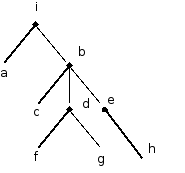
\includegraphics[height=120pt, width=180pt]{Arbre1.png}} 2. \frame{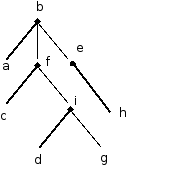
\includegraphics[height=120pt, width=180pt]{Arbre2.png}}\\\\
3. \frame{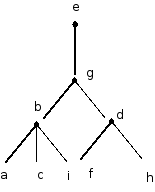
\includegraphics[height=120pt, width=180pt]{Arbre3.png}} 4. \frame{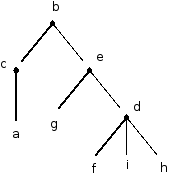
\includegraphics[height=120pt, width=180pt]{Arbre4.png}}\\\\
5. \frame{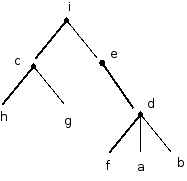
\includegraphics[height=120pt, width=180pt]{Arbre5.png}} 6. \frame{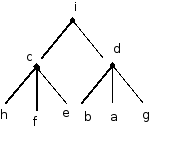
\includegraphics[height=120pt, width=180pt]{Arbre6.png}}\\\\

\subsection{Réponses}
\begin{enumerate}
    \item (i (a) (b (c) (d (f) (g)) (e (h))))
    \item (b (a) (f (c) (i (d) (g))) (e (h)))
    \item (e (g (b (a) (c) (i)) (d (f) (h))))
    \item (b (c (a)) (e (g) (d (f) (i) (h))))
    \item (i (c (h) (g)) (e (d (f) (a) (b))))
    \item (i (c (h) (f) (e)) (d (b) (a) (g)))
\end{enumerate}

\section{Conversion de listes en arbres}
\subsection{Question}
Voici quelques représentations internes d'arbres sous forme de listes ; à l'aide de Dia, en utilisant la feuille Arbre, tracez leur représentation externe (sous forme de schéma) :
\begin{enumerate}
    \item (a (b (c (d) (e) (f)) (g (h)) (i)))
    \item (b (i (d) (e) (f (g (h)) (c))) (a))
    \item (a (i (c (b (e (h))) (g (d)) (f))))
    \item (a (d (e (b (c (f))) (g)) (i)) (h))
    \item (i (b (e (h)) (a)) (f) (c) (d (g)))
    \item (h (f (g (b)) (i (d) (e)) (c (a))))
\end{enumerate}

\subsection{Réponses}
\begin{enumerate}
    \item -\\ 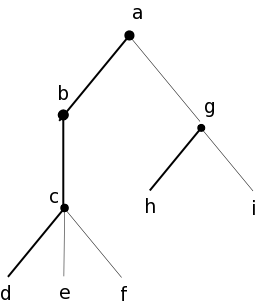
\includegraphics[scale=0.3]{reponse1.png}
    \item -\\ 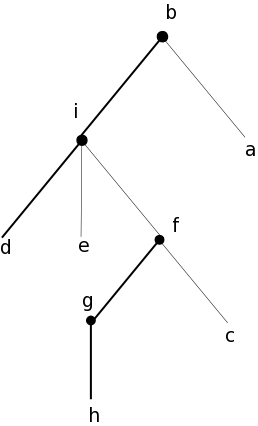
\includegraphics[scale=0.3]{reponse2.png}
    \item -\\ 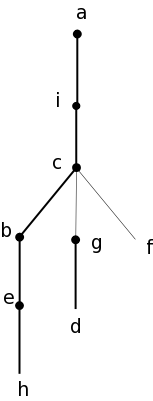
\includegraphics[scale=0.3]{reponse3.png}
    \item -\\ 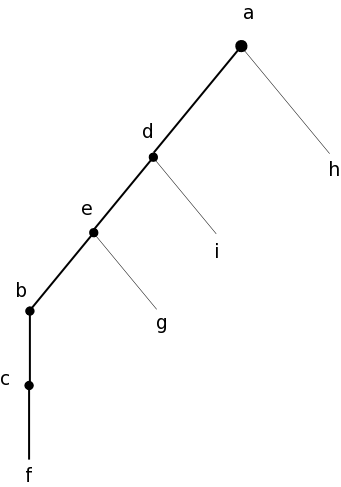
\includegraphics[scale=0.3]{reponse4.png}
    \item -\\ 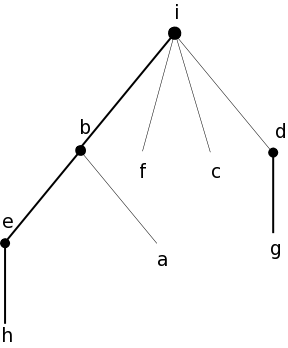
\includegraphics[scale=0.3]{reponse5.png}
    \item -\\ 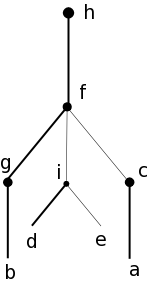
\includegraphics[scale=0.3]{reponse6.png}
\end{enumerate}
%
\end{document}

